 \documentclass[12pt]{article}
 \usepackage{url}  % Formatting web addresses
 \usepackage[round,sort]{natbib}
 \usepackage{graphicx}
 \usepackage{amsbsy}
 \usepackage{amsmath}
 \usepackage{pdflscape}
\usepackage{verbatim}
\usepackage{fullpage}
 \graphicspath{{graphics/}}
 \usepackage[pdfborder={0 0 0},pdftex]{hyperref}
 \usepackage{setspace}
\usepackage[affil-it]{authblk}
\pdfminorversion=5
\nonstopmode
%\usepackage{endfloat}
\usepackage{lineno}
%\doublespacing


 \begin{document}
 \title{Estimating Uncertainty in Daily Weather Interpolations: a
   Bayesian Framework for Developing Climate Surfaces}

 \author{Adam M. Wilson}
\affil{\small Department of Ecology and Evolutionary Biology \\
  University of Connecticut, Storrs, CT \\ \medskip
Current Address: \\
Department of Ecology and Evolutionary Biology \\
165 Prospect St. \\
Yale University\\ 
New Haven, CT  06520 \\
Telephone: +1 (203)-432-7540 \\
Fax: +1 (203) 432-5176\\
Email: adam.wilson@yale.edu}

\author{John A. Silander, Jr.}
\affil{\small Department of Ecology and Evolutionary Biology \\ University of Connecticut, Storrs, CT}

 \maketitle

\newpage
Short Title: Uncertainty in Daily Weather Interpolations

\linenumbers
\begin{abstract}
Conservation of biodiversity demands comprehension of evolutionary and
ecological patterns and processes that occur over vast spatial and
temporal scales. 
A central goal of ecology is to understand the climatic factors that control
ecological processes and this has become even more
important in the face of climate change.  
Especially at global scales, there can be enormous
uncertainty in underlying environmental data used to explain
ecological processes, but that uncertainty
is rarely quantified or incorporated into ecological models.  
In this study a climate-aided Bayesian kriging approach is used to
interpolate 20 years of daily meteorological
observations (maximum and minimum temperature and precipitation) to a
1 arc-minute grid for the Cape Floristic Region of
South Africa.  Independent validation data revealed overall predictive
performance of the interpolation to have R$^2$ values of 0.90, 0.85, and 0.59
for maximum temperature, minimum temperature, and precipitation, respectively.
A suite of ecologically-relevant climate metrics that include the
uncertainty introduced by the interpolation were then generated. 
By providing the high resolution climate metric surfaces and uncertainties, this work
facilitates richer and more robust predictive modeling in ecology and biogeography.  
These data can be incorporated into ecological models to propagate the uncertainties
through to the final predictions.  

\end{abstract}
\medskip
{\bf Keywords:} interpolation, bayesian, krige, climate metric, ecology \\
{\bf Acknowledgments:} This work was supported by NSF grants OISE-0623341, DEB-0516320, and DEB-1046328 to JAS and by NASA headquarters under the NASA Earth and Space Science Fellowship Program grant NNX09AN82H to AMW.   We also thank Chris Lennard and Lisa Coop at the Climate System Analysis Group at the University of Cape Town for providing the station data.
 \newpage
\section{Introduction}
\doublespacing

The role of climate in driving ecological processes has been known for
170$^+$ years \citep[\textit{e.g.}][]{meyen_outlines_1846}. 
Recently, in the face of climate change, the scientific
community has focused its attention on the role of climate and weather
in ecological processes, evident in the thousands of publications on
the topic since the year 2000.   A limiting factor for many ecological
studies is the availability of accurate weather and climate data for locations of interest \citep{hijmans_very_2005}.
Unfortunately for this purpose, weather stations are often irregularly spaced and
clustered in heavily populated, low elevation areas which may be far from where
ecological observations are made or needed. 
Thus ecologists are faced with the problem of estimating  weather/climate for the locations of interest.
For many types of analysis, gridded weather/climate data are
preferable to point observations because of their spatial continuity
\citep{haylock_european_2008} and several methods exist for interpolating from station observations to a
continuous surface across the region including: nearest neighbor
\citep{stahl_comparison_2006}, Cressman Interpolation
\citep{cressman_operational_1959}, thin-plate splines
\citep{tait_thin_2006}, generalized additive models
\citep{guan_modeling_2009}, and kriging
\citep{haylock_european_2008}. See \citealp{apaydin_spatial_2004} for a
review of other methods.

This study was motivated by two concerns:
\begin{itemize}
\item Ecologists often use output from meteorological and climatological analysis as input for  their models without
  incorporating the uncertainty inherent in the climate product.  
\item Most climate data used in ecological models are coarse temporal
  aggregations such as monthly means rather than variables that are
  known to be more relevant to the ecological process under study,
  such as the longest period between rain events or absolute minimum temperature.
\end{itemize}

\subsection{Estimating Uncertainty}

Scientists are under increasing pressure to improve estimates of
uncertainty in both ecology
\citep[\textit{e.g.}][]{cressie_accounting_2009} and climate change research \citep[\textit{e.g.}][]{collins_towards_2006}.  
Ecologists often use climatological and meteorological model output
as input to their analysis as if they
were `truth' despite evidence that the results can vary widely
depending on which data are used
\citep{soria-auza_impact_2010,roubicek_does_2010,peterson_environmental_2008,wiens_niches_2009}. 
For example, it is not uncommon to build species
distribution models that treat interpolated climate surfaces as data and ignore any
uncertainty inherent in the surfaces \citep[\textit{e.g.}][]{raes_botanical_2009,williams_using_2009,ward_modelling_2007,pearson_predicting_2007}. 
Furthermore, producers of climate data often share only the 'best estimates' of
the quantities of interest \citep{daly_guidelines_2006} making incorporation of the uncertainty
impossible.  Perhaps the most commonly cited ($>2,000$
citations as of July 2013) example of this
is the WorldClim data set which offers 30
arc-second ($\sim$1km) resolution globally whether
the pixel contains a weather station or the nearest station is
hundreds of kilometers away \citep{hijmans_very_2005}.  
The value of an interpolated 1km pixel that is hundreds of
kilometers from the nearest weather station (a common situation
throughout the tropics) is much less certain than that of
a pixel  located at a weather station, but without any reported
uncertainty,  one is led to the  biased conclusion that the spatial
accuracy of the product is uniform.   Furthermore, the increased
availability of very fine climate surfaces can lead the user to ``equate resolution with realism''
despite the importance of fine-scale
climatological process that are not represented in the interpolation
algorithm \citep{daly_guidelines_2006}.
As ecological models become more complex, it is vital to account for
uncertainty inherent in data and propagate it through to
the results \citep{luo_ecological_2011,clark_future_2006}.

\subsection{Climate Metrics}

There is growing awareness that organisms may respond more to
climate extremes and other climate metrics (such as annual minimum temperature, growing season length, and the longest
annual period between precipitation events) than mean values
\citep{gutschick_extreme_2003,trnka_agroclimatic_2011,jackson_ecology_2009}. However
these more proximal metrics are more difficult to calculate because they
generally require daily (or more frequent) meteorological observations.  
The use of coarse aggregate metrics, such as monthly means, is
typically supported with the argument that they tend to be correlated with more
proximal variables across space \citep{jackson_ecology_2009}.
However, when the goal is prediction of ecological processes, such as phenology
\citep[e.g.][]{richardson_phenology_2006}, demographics
\citep[e.g.][]{colchero_predicting_2009,clark_uncertainty_2003}, or
disturbance \citep[e.g.][]{wilson_hierarchical_2010} into new areas or times, models that capture more direct mechanistic
relationships are likely to have better predictive performance
\citep{jackson_ecology_2009}.
Furthermore, global change may lead to a temporal decoupling
between the aggregate measures and the more proximal variables that
directly affect the ecological process of interest
\citep{jackson_ecology_2009}.  

As many of these metrics are sensitive to daily meteorological events, ignoring the uncertainty in each day's predictions
makes it impossible to estimate uncertainty in the metrics or in any
subsequent analysis. 
For example, the longest annual dry spell could be cut in half by a
single rain event.
Methods that result in a single-valued prediction for rainfall on a
given day will result in a single estimate of the longest annual dry
spell with no accounting for the uncertainty in each day's
rainfall prediction, regardless of the distance to the nearest station.
It is thus difficult, if not impossible, to estimate uncertainty in these metrics using
traditional interpolation methods that result in only 'best estimates' of daily weather.  

\subsection{Bayesian Solution}

Bayesian methods are capable of generating a full posterior distribution of all unknown
model parameters \citep{clark_why_2004} and are becoming more common in climatological
analyses \citep[e.g.][]{fischer_climate_2012,iizumi_statistical_2012,ruggieri_bayesian_2013}.  
Thus a Bayesian interpolation results in a
distribution of meteorological values for each prediction location for
each time.  
It is possible to sample from these distributions of daily meteorology
and generate any climate metric of interest.
For example, we can draw 1,000 precipitation values from each day's
posterior distribution for a given year and calculate 1,000
realizations of length of the longest dry spell.  From this
distribution, any summary of interest (such as the mean or variance) can be derived with credible intervals.

In this study a framework is presented to interpolate daily station
weather data (maximum and minimum temperature and precipitation) to
high resolution surfaces, calculate relevant climate metrics
\citep[see ][for a discussion of selecting relevant metrics for plants]{kimball_fitness_2012}, and keep track of the
uncertainties introduced by the interpolation.
For simplicity, in this paper the interpolated surfaces of
daily weather data are referred to as `meteorological' surfaces and the derivative
metrics (such as growing degree days) as yearly `climate metrics,' even
though they are not long-term (multi-decadal) aggregations.
The yearly `climate metrics' could be further processed to produce
typical climatologies that summarize the parameter over many years
(\textit{e.g.} the 30-year distributions of annual growing degree days).
While other studies have used Bayesian methods to interpolate
meteorological surfaces
\citep{sang_hierarchical_2009,cooley_bayesian_2007,riccio_bayesian_2005,newlands_validation_2011,johansson_high-resolution_2008,
alvarez-villa_improved_2011,fasbender_spatial_2010},  to our knowledge this is
the first effort to use the posterior distributions to generate
surfaces of ecologically-relevant climate metrics that incorporate the
uncertainty introduced by the interpolation process. 

\section{Methods}
\subsection{Study Area}
The Cape Floristic Region (CFR) of South
Africa ($\sim$90,000 km$^2$) is home to almost 9,000
species, 65\% of which are endemic \citep{goldblatt_floristic_1997}.
Species in the CFR tend to be locally abundant but have small
ranges and limited dispersal capabilities
\citep{latimer_neutral_2005}. 
These factors suggest that the region's biodiversity may be sensitive to
shifts in the precipitation regime predicted under future climate
change \citep[][section 11.2.3]{christensen_chapter_2007}.   
The region is topographically and climatically diverse, with
elevations ranging from sea level to over 2,000m and mean
annual rainfall ranging from 60mm to greater than 3,300mm
\citep{schulze_south_2007}.  
In this study, we interpolate 20 years (1990-2010) of daily weather (maximum
temperature, minimum temperature, and precipitation) observations to a
1 minute ($\sim$1.55km x 1.85km) grid for the CFR.  

\subsection{Modeling}
Large, topographically heterogeneous regions present challenges for
interpolation of weather, especially precipitation.  Several recent
studies have revealed that interpolating anomalies of
daily weather from long-term or monthly means rather
than the raw, observed values can lead to improved prediction accuracy
\citep[\textit{e.g. }][]{haylock_european_2008,hunter_climatologically_2005}.
The framework described in these studies was used to calculate the daily
anomolies for each station from long-term climate surfaces as follows for precipitation:

\begin{equation}
P_{\text{anomaly}}=\frac{P_{\text{daily}}}{P_{\text{monthly}}} \label{eq:ppttrans}
\end{equation}

and temperature:
\begin{equation}
T_{\text{anomaly}}=T_{\text{monthly}}-T_{\text{daily}} \label{eq:temptrans}
\end{equation}

Classical geostatistical inference (Kriging) treats interpolation as two
separate steps, parameter estimation and prediction
\citep{diggle_model-based_2007}.  
In common practice, the best estimate of the
interpolation parameters is ``plugged in'' as if it were truth and the
uncertainty in the model parameters is not propagated through to the prediction variance.
This procedure often leads to an overestimate of the certainty of the
predictions.  To overcome this limitation, we applied the 'bayesian
krige' described by Diggle and Ribeiro (\citeyear[][Section 7.2.3]{diggle_model-based_2007}).  
This approach treats the kriging parameters: the sill ($\sigma^2$) ,
range ($\phi$), and nugget ($\tau$) as random variables
and thus the predictive distribution incorporates their
uncertainty (Figure \ref{fig:kriging}). In addition, like co-kriging, the model also allows
additional co-variates (${\bf X}$) to be included in a regression framework.  Because the response data are daily anomalies from the mean (rather than the absolute daily values), there is little fine-grain variability corresponding to local environmental conditions (such as elevation).  In other words, a day that is colder than average tends to be colder than average both at the top and the bottom of a mountain.  In this study we include both latitude and longitude to allow linear trends in both dimensions. The coefficients for these variables are represented by ${\boldsymbol \beta}$.
The model can be written as follows, where $({\bf u})$ represents locations \citep[from][Section 4.5]{ribeiro_jr_bayesian_2009}:

\begin{gather}
\mathbf{Y(u)}= \mathbf{X\boldsymbol{\beta}}+\sigma T({\bf
  u})+\varepsilon({\bf u})\\
T({\bf u})\sim\mathcal{N}(0,R(\phi)) 
\hspace{10pt} \text{and} 
\hspace{10pt} \varepsilon\stackrel{\mathrm{i.i.d}}{\sim}\mathcal{N}(0,\tau^2)
\end{gather}
consequently,
\begin{equation}
pr(Y|\boldsymbol{\beta},\sigma^2,\phi,\tau^2_R)\sim
\mathcal{N}\big(X\boldsymbol{\beta},\sigma^2R(\phi,\tau^2_R)\big)
\end{equation}
where
\begin{equation}
R(\phi,\tau^2_R)=\sigma^2\big[R(\phi)+\tau^2_R\mathcal{I}\big]=\sigma^2\Big[R(\phi)+\frac{\tau^2}{\sigma^2}\mathcal{I}\Big].
\end{equation}


\begin{figure}
  \begin{center}
 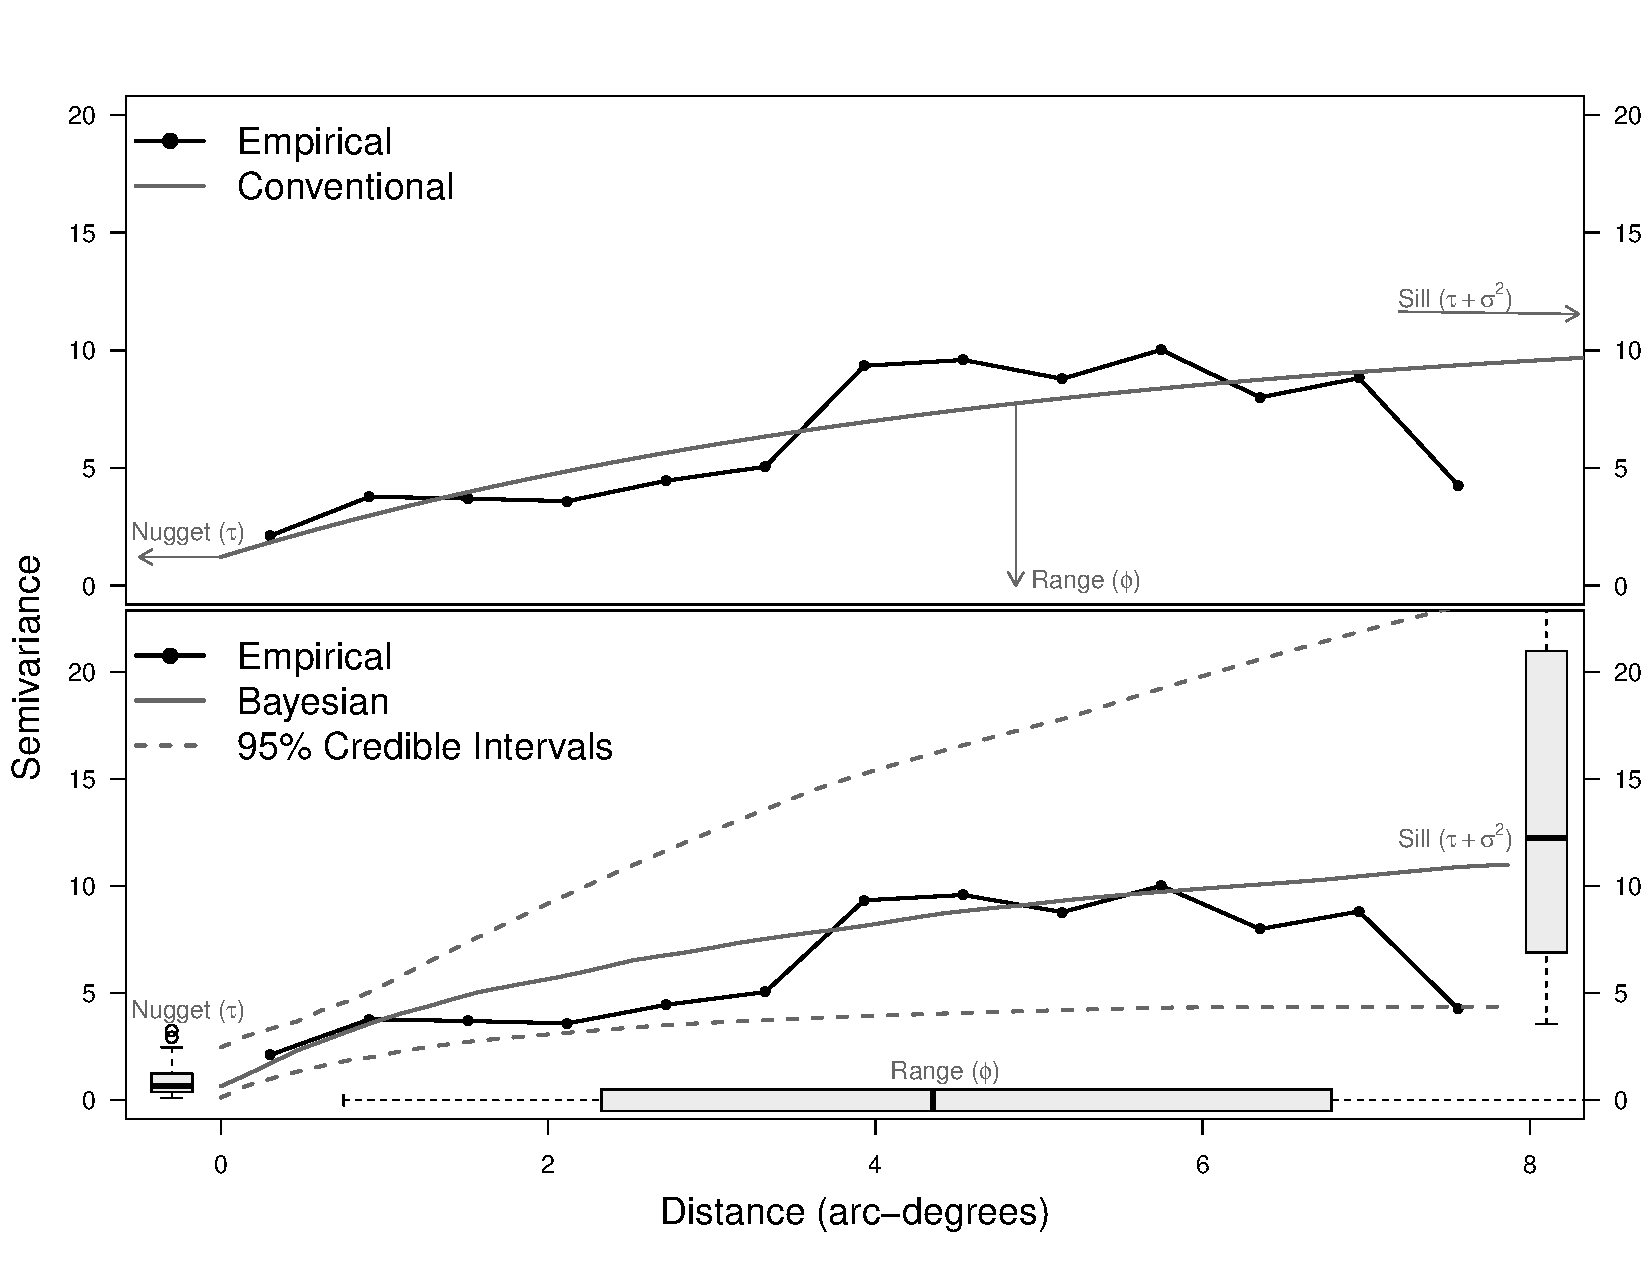
\includegraphics[width=\textwidth]{Figure1.pdf} \caption{Empirical
   (black) and fitted (grey) semivariograms for maximum temperature on
   January 3, 2009. The top panel shows the variogram and spatial
   parameters fitted using conventional techniques, while the bottom
   panel shows the Bayesian variogram with 95\% credible intervals. The box plots on the X and Y axis represent the
   posterior distributions of the three spatial parameters: the sill ($\sigma^2$) ,
range ($\phi$), and nugget ($\tau$).  Note that the median Bayesian
curve is very similar to the conventional variogram, but the Bayesian
method quantifies the uncertainty in the variogram due to uncertainty
in the kriging parameters.}
    \label{fig:kriging}
\end{center}
\end{figure}




We used the \texttt{krige.bayes} function in the \texttt{geoR} package
\citep{diggle_geor:_2001} of R \citep[][v2.12.1]{r_development_core_team_r:_2011}
to perform the day-by-day interpolations.  
This function simplifies model fitting with
discretized prior distributions for $\phi$ and the 'noise to signal
variance ratio' ($\tau^2_R=\frac{\tau^2}{\sigma^2}$).  
A discretized reciprocal
prior was used for $\sigma^2$ and $\frac{\tau^2}{\sigma^2}$ and a discretized  exponential
prior was used for $\phi$ \citep[see ][for a discussion of various choices for
these parameters]{diggle_bayesian_2002}.

The prediction of the daily anomalies was done on a $^1/_4$ degree
grid which was then down-sampled to the 1-minute climate grid using a
bi-cubic resampling algorithm. Computational limitations prevented making the
predictions at the full one minute resolution (see Section
\ref{sec:comp}).  However, as anomaly surfaces are ``relatively free of the
considerable topography-forced spatial variability,''
\citep{willmott_climatologically_1995} the surfaces at $^1/_4$
degree are relatively smooth.  The high resolution
anomaly surfaces were then converted back to the original units ($^o$C
for temperature and mm for precipitation) by inverting the relationships in Equations \ref{eq:ppttrans} and \ref{eq:temptrans}.

\subsection{Data}
Daily weather observations were collected from $\sim$700 weather
stations (70 temperature and 645 precipitation) across the region
(Figure \ref{fig:wmap}) by the South African Weather
Service (SAWS, \url{http://www.weathersa.co.za/}) and the South
African Computing Center for Water Research (University of Natal, P/Bag X01, Scottsville 3209, South Africa). 
These data were assembled and quality controlled by the Climate Systems Analysis
Group at the University of Cape Town (CSAG,
\url{http://www.csag.uct.ac.za/}) based on measures used by the daily
Global Historical Climate Network \citep{williams_united_2006}.  
We used long-term monthly climate surfaces of mean monthly maximum and minimum
temperature and total precipitation.  
These surfaces were developed from quality controlled station
observations from the period for 1950-2000 as
described in \cite{schulze_south_2007}.  
These  high resolution climate surfaces facilitated incorporation of spatial and
temporally varying lapse rates that are based on $>$50-year time series
and other sources of information (see \citealp{schulze_south_2007}, for
details).  

\begin{figure}
  \begin{center}
 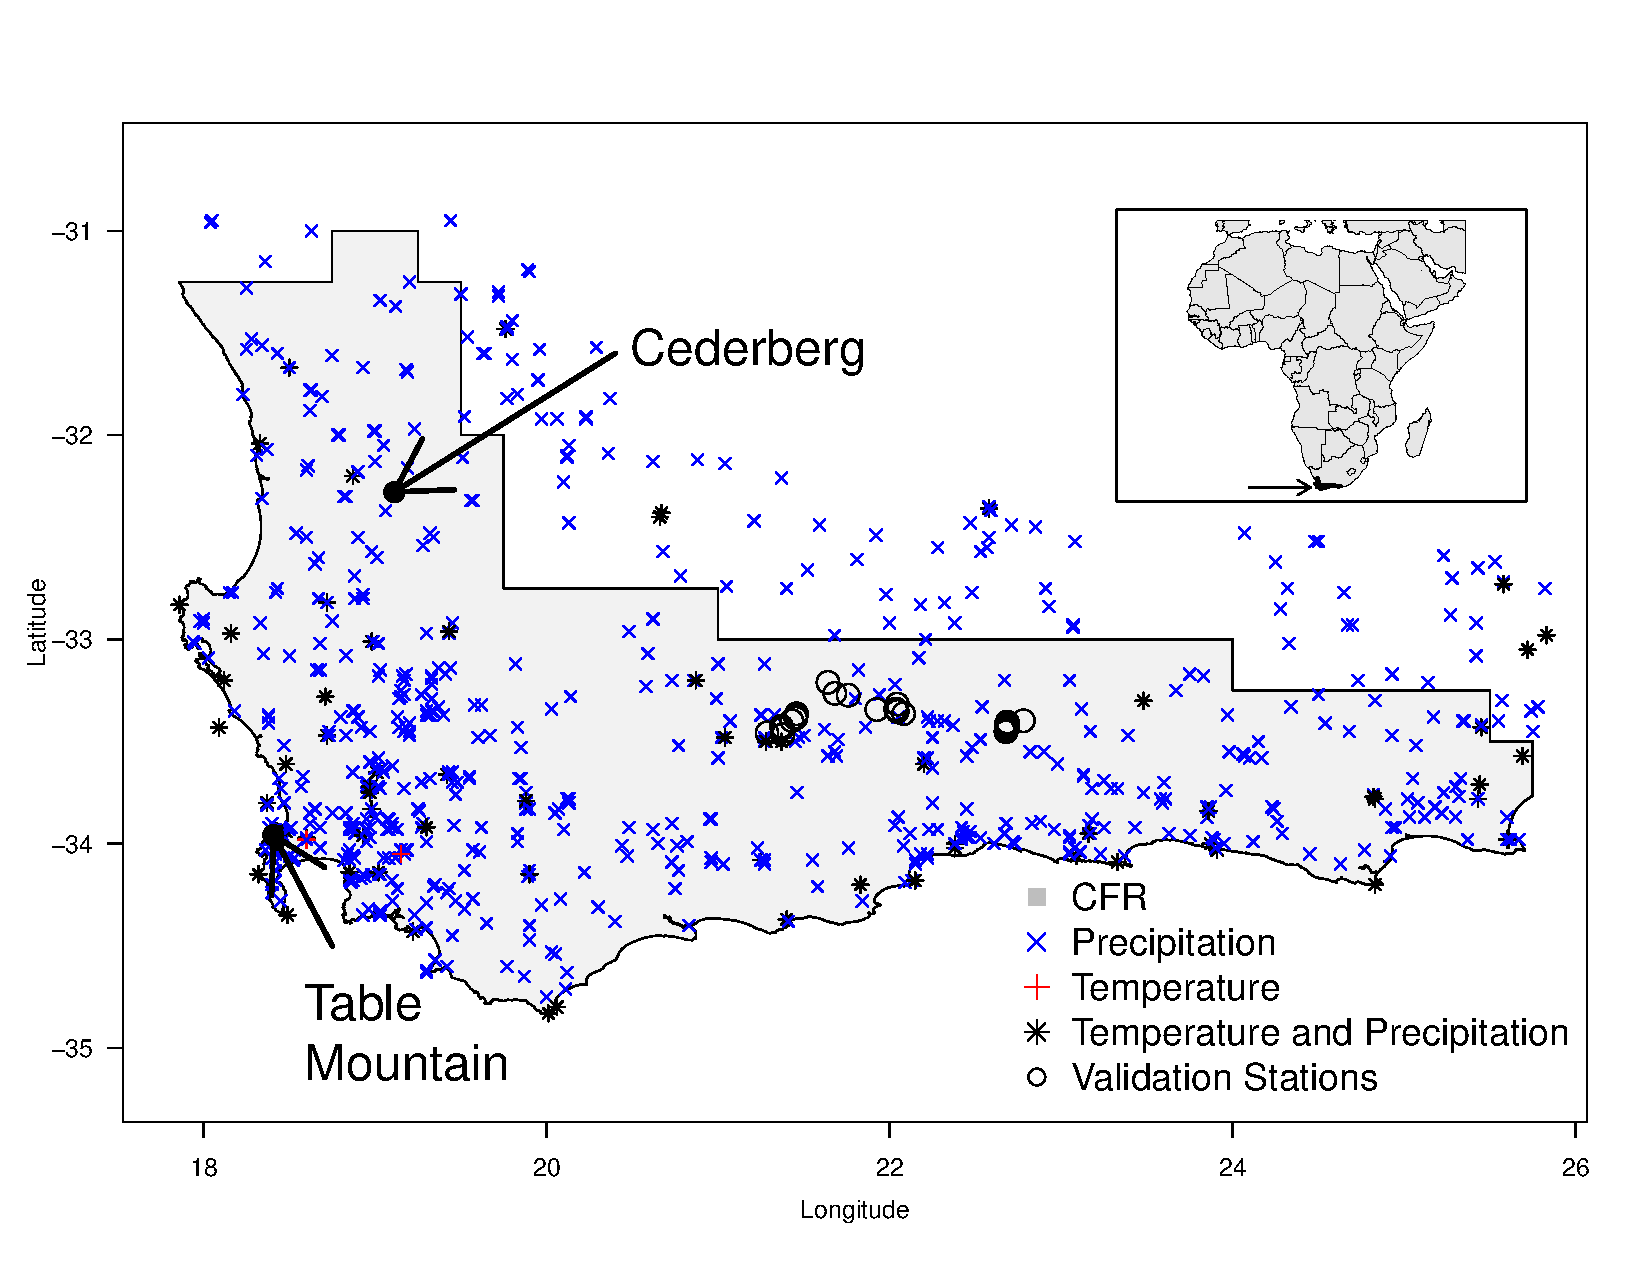
\includegraphics[width=\textwidth]{Figure2.pdf} \caption{Map
   of the Cape Floristic Region (CFR, in gray) of South Africa showing locations of
   various types of weather stations included in this study.  Stations
   within 75km of the CFR were included to aid in interpolation near
   the edges of the region. The validation stations are locations with
   monthly data that were not included in the interpolation.  
   Filled circles show locations of the two example
   locations discussed in the text. 
   Inset shows location of the CFR within Africa.}
    \label{fig:wmap}
\end{center}
\end{figure}


\subsection{Climate Metrics}

A set of climate metrics was selected to target various aspects of
plant performance in the CFR (Table \ref{tab:climmet}). For example,
seedling survival in the region is sensitive to summer drought
\citep{midgley_mortality_1988}, which was quantified by the length of the
longest dry spell, and germination of some species may require
stratification by sufficiently cold minimum temperatures
\citep{keeley_convergent_1997}, which is quantified with the absolute
minimum temperature of the year.   The other biologically relevant metrics are summarized in Table \ref{tab:climmet}. 
The climate metrics were calculated for each location using a time series consisting of samples from each day's posterior
distribution for each year.  
This process resulted in a posterior distribution
for each climate metric, for each pixel, for each year.  
These distributions were then summarized to derive the mean, standard
deviation and credible intervals of the predicted metrics.  

\subsection{Validation}
The models were evaluated in two ways.  
During model
fitting,  observations from three randomly
selected stations were held out each day.
Three stations were selected to ensure some spatial coverage for each
day without impacting the performance of the model.
This sub-setting resulted in over 20,000 validation observations that were not used in model fitting.  
The mean posterior predictions for these locations were then compared with the observed
data to assess the predictive accuracy using the coefficient of
determination, root mean square error, mean absolute error, and mean
error.  In addition, for precipitation, the model's ability to predict
`wet days' where $ppt\ge2mm$ was assessed using the positive predicted
value (\% predicted wet that were wet)
and negative predicted value (\% predicted dry that were dry).

The second evaluation was to calculate monthly maximum and minimum temperature and
monthly total precipitation for additional locations in the study area
where monthly total precipitation and monthly minimum and maximum
temperature are available (Figure \ref{fig:wmap}).  
These stations, maintained by the CapeNature Management organization (\url{http://www.capenature.co.za/}) are all in mountainous areas and represent the most
difficult prediction locations and are thus useful for evaluating the product for use in these
remote regions.  
This validation is also useful to assess any temporal bias resulting from
modeling each day independently.  

\subsection{Computational Notes} \label{sec:comp}
Fitting the daily models in this framework is computationally
demanding in terms of both storage and processing.  
The models were run on a cluster of 74 Xeon E5530 2.4GHz
quad-core hyper-threading CPUs at the University of California Davis (making $>$500 threads available for
processing).  Processing the 20 years of data required $\approx$200 processor days to complete.
The posterior samples for each day were converted to netCDF v4.0
format and summarized with the NCAR Climate Language
\citep{national_center_for_atmospheric_research_ncar_2011}, the NetCDF Climate Operators
\citep{zender_analysis_2008}, and the Climate Data Operators
\citep{mueller_climate_2013} using R
\citep{r_development_core_team_r:_2011} as the overall scripting
language.  
The full posterior dataset (consisting of 1000 iterations of maximum and minimum
temperature and precipitation at 1 minute resolution for each day) requires over 7 terabytes of disk space. 


\section{Results}

\subsection{Validation of Daily Data}

%% latex table generated in R 2.13.1 by xtable 1.6-0 package
% Tue Oct 18 15:50:02 2011
\begin{table}[ht]
\begin{center}
\begin{tabular}{lrrrrr|rrrrr}
  \hline & \multicolumn{5}{c|}{Daily data} & \multicolumn{5}{c}{Monthly data} \\ \hline
Variable & RMSE & MAE & MER & R$^2$ & n  & RMSE & MAE & MER & R$^2$ & n \\ 
  \hline
Maximum Temperature ($^o$C) & 1.79 & 1.26 & -0.03 & 0.90 & 21,915 & 4.93 & 3.79 & 0.67 & 0.60 &1,280\\ 
  Minimum Temperature  ($^o$C) & 1.73 & 1.26 & -0.06 & 0.85 & 21,915 &
  3.39 & 2.67 & 1.02 & 0.48 & 1,138 \\ 
  Precipitation (mm) & 3.92 & 0.85 & -0.02 & 0.59 & 21,915 & 29.61 &
  19.71 & -3.60 & 0.56 & 5,036\\ 
   \hline
\end{tabular}
\caption{Validation results for each variable.  The comparison of daily data are from the daily observations not included in model fitting. The monthly data compare predicted and observed total monthly precipitation and monthly maximum and minimum temperature at a set of remote stations.  The poorer fit for the monthly temperature is expected as it represents the ability of the model to estimate the single daily maximum and minimum in each month, while the monthly precipitation comparison is the aggregated total for the month. The validation metrics are as follows. RMSE: Root Mean Squared Errors, MAE: Mean Absolute Error, MER: Mean Error}
\label{tab:valid}
\end{center}
\end{table}


\begin{figure}
  \begin{center}
 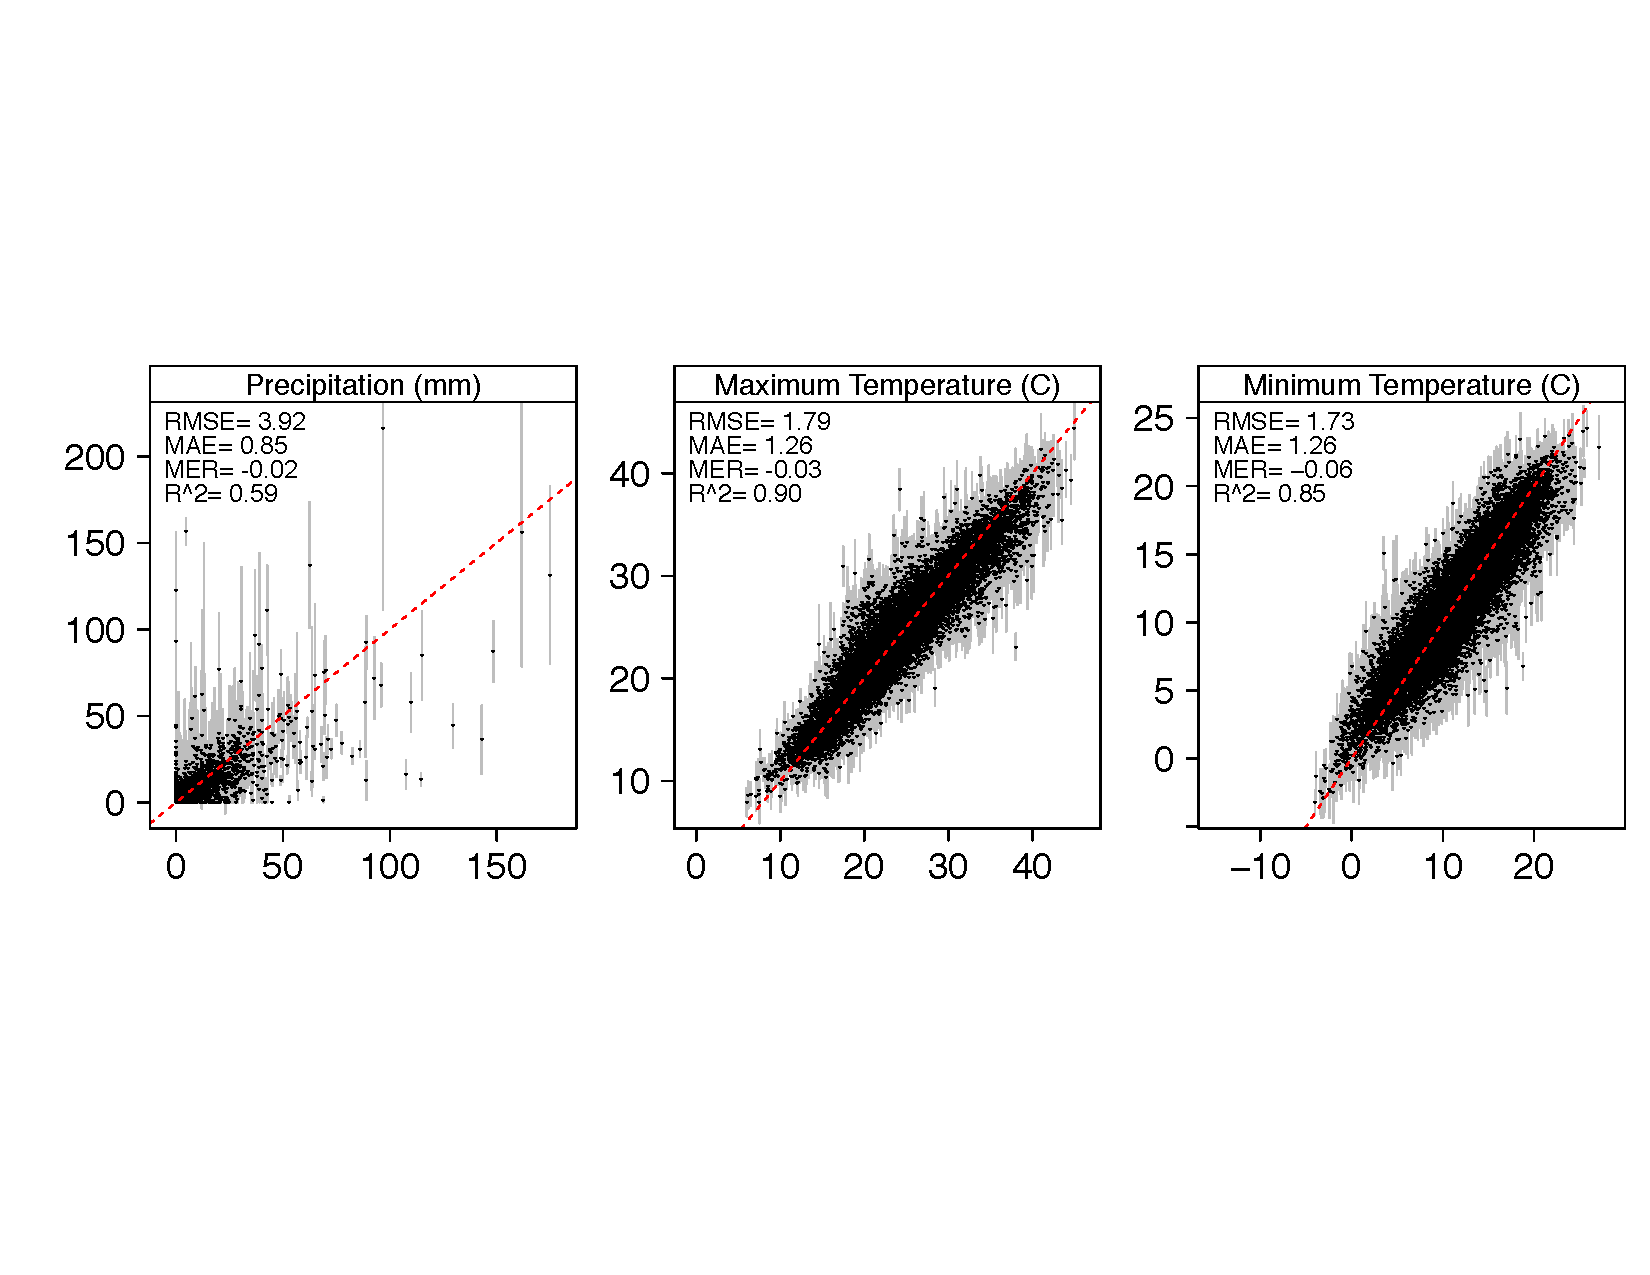
\includegraphics[clip=true,trim= 0 5.2mm 0 5.4mm,width=\textwidth]{Figure3.pdf} \caption{Scatterplot of
   predicted and observed weather from the three hold-out validation
   observations from each day during 1990--2009 (totaling
   $\approx$20,000 observations).  The units for both $x$ and $y$ axis
   are $^o$C for temperature and mm for precipitation.
   Grey bars represent $\pm1$ standard deviation of the posterior
   distributions. The dashed lines indicate $y=x$. 
   The validation metrics are as follows; RMSE: Root Mean Squared Errors, MAE: Mean Absolute Error, MER: Mean Error}
    \label{fig:predobs}
\end{center}
\end{figure}

Overall, the model achieved high predictive accuracies for
daily minimum and maximum temperature (R$^2=0.85$ and R$^2=0.90$,
respectively), and moderate accuracy for precipitation (R$^2=0.59$)
(Figures \ref{fig:predobs}, \ref{fig:predobsm}, and Table \ref{tab:valid}).
The mean absolute errors were generally low for all variables
(1.26$^oC$ for both maximum and minimum temperature,
and 0.85mm for precipitation).  The model successfully predicted dry
days ($\le2mm$) 97\% of the time and wet days 66\% of the time.
Figure \ref{fig:predobsm} shows the predicted vs. observed
scatterplots grouped by month.  The predictive accuracy is relatively
similar throughout the year.

%\begin{landscape}  %several landscape pages

\begin{table}[left]
\begin{small}
  \begin{tabular}{p{1.6cm}|p{4cm}|p{3.5cm}|p{1cm}|p{6cm}}
    \hline
    Quantity & Description & Plant performance elements & Input Data & Functional form\\
    \hline
    MinT & Annual minimum temperature & Seed stratification, germination,    growth &  $t_{min}$ & min$(t_{min})$\\
   MaxT & Annual maximum temperature & Germination, growth, Seedling mortality &  $t_{max}$ & max$(t_{max})$\\
 
   FD & Frost days & Seedling mortality & $t_{min}$ & $\sum_{t\in\text{year}}(t_{min_t}<0^oC)$\\
    CFD & Longest consecutive period with frost & Seedling mortality & $t_{min}$ &
    max(consecutive($t_{min}<0^oC$))\\
    GDD & Growing Degree Days & Growth & $t_{max}$ &$\sum_{t\in\text{year}}\text{max}(t_{min_t}-10.0)$\\
    CSU & Consecutive Summer Days ($>35^oC$) & Seedling mortality & $t_{max}$ & max(consecutive($t_{max}>35^oC$))\\
      CDD & Annual maximum consecutive dry days & Growth, Seedling
    mortality & $ppt$ & max(consecutive($ppt<$2mm))\\
    ECA & Very heavy precipitation days & Growth,
   Seedling mortality & $ppt$ & Number of days with $ppt>$20mm \\
   SDII & Simple daily precipitation intensity index & Growth,
   Seedling mortality & $ppt$ & mean($ppt$) where $ppt>$2mm\\
  \end{tabular}
\end{small}
  \caption{Climate metrics were calculated using 1,000 time series
    drawn from the posterior samples in each location to result in a
    posterior distribution that incorporates the uncertainty
    introduced by the interpolation. Climate metrics were calculated
    using CDO tools \citep{mueller_climate_2013}.}
  \label{tab:climmet}
\end{table}


%\newpage
\begin{table}[ht]
\begin{center}
\begin{footnotesize}
\begin{tabular}{lrrrrr|rrrrr}
  \hline & \multicolumn{5}{c|}{Daily data} & \multicolumn{5}{c}{Monthly data} \\ \hline
Variable & RMSE & MAE & MER & R$^2$ & n  & RMSE & MAE & MER & R$^2$ & n \\ 
  \hline
Maximum Temperature ($^o$C) & 1.79 & 1.26 & -0.03 & 0.90 & 21,915 & 4.93 & 3.79 & 0.67 & 0.60 &1,280\\ 
  Minimum Temperature  ($^o$C) & 1.73 & 1.26 & -0.06 & 0.85 & 21,915 &
  3.39 & 2.67 & 1.02 & 0.48 & 1,138 \\ 
  Precipitation (mm) & 3.92 & 0.85 & -0.02 & 0.59 & 21,915 & 29.61 &
  19.71 & -3.60 & 0.56 & 5,036\\ 
   \hline
\end{tabular}
\end{footnotesize}
\caption{Validation results for each variable.  The comparison of daily data are from the daily observations not included in model fitting. The monthly data compare predicted and observed total monthly precipitation and monthly maximum and minimum temperature at a set of remote stations.  The poorer fit for the monthly temperature is expected as it represents the ability of the model to estimate the single daily maximum and minimum in each month, while the monthly precipitation comparison is the aggregated total for the month. The validation metrics are as follows. RMSE: Root Mean Squared Errors, MAE: Mean Absolute Error, MER: Mean Error}
\label{tab:valid}
\end{center}
\end{table}



%\newpage
\begin{figure}
  \begin{center}
 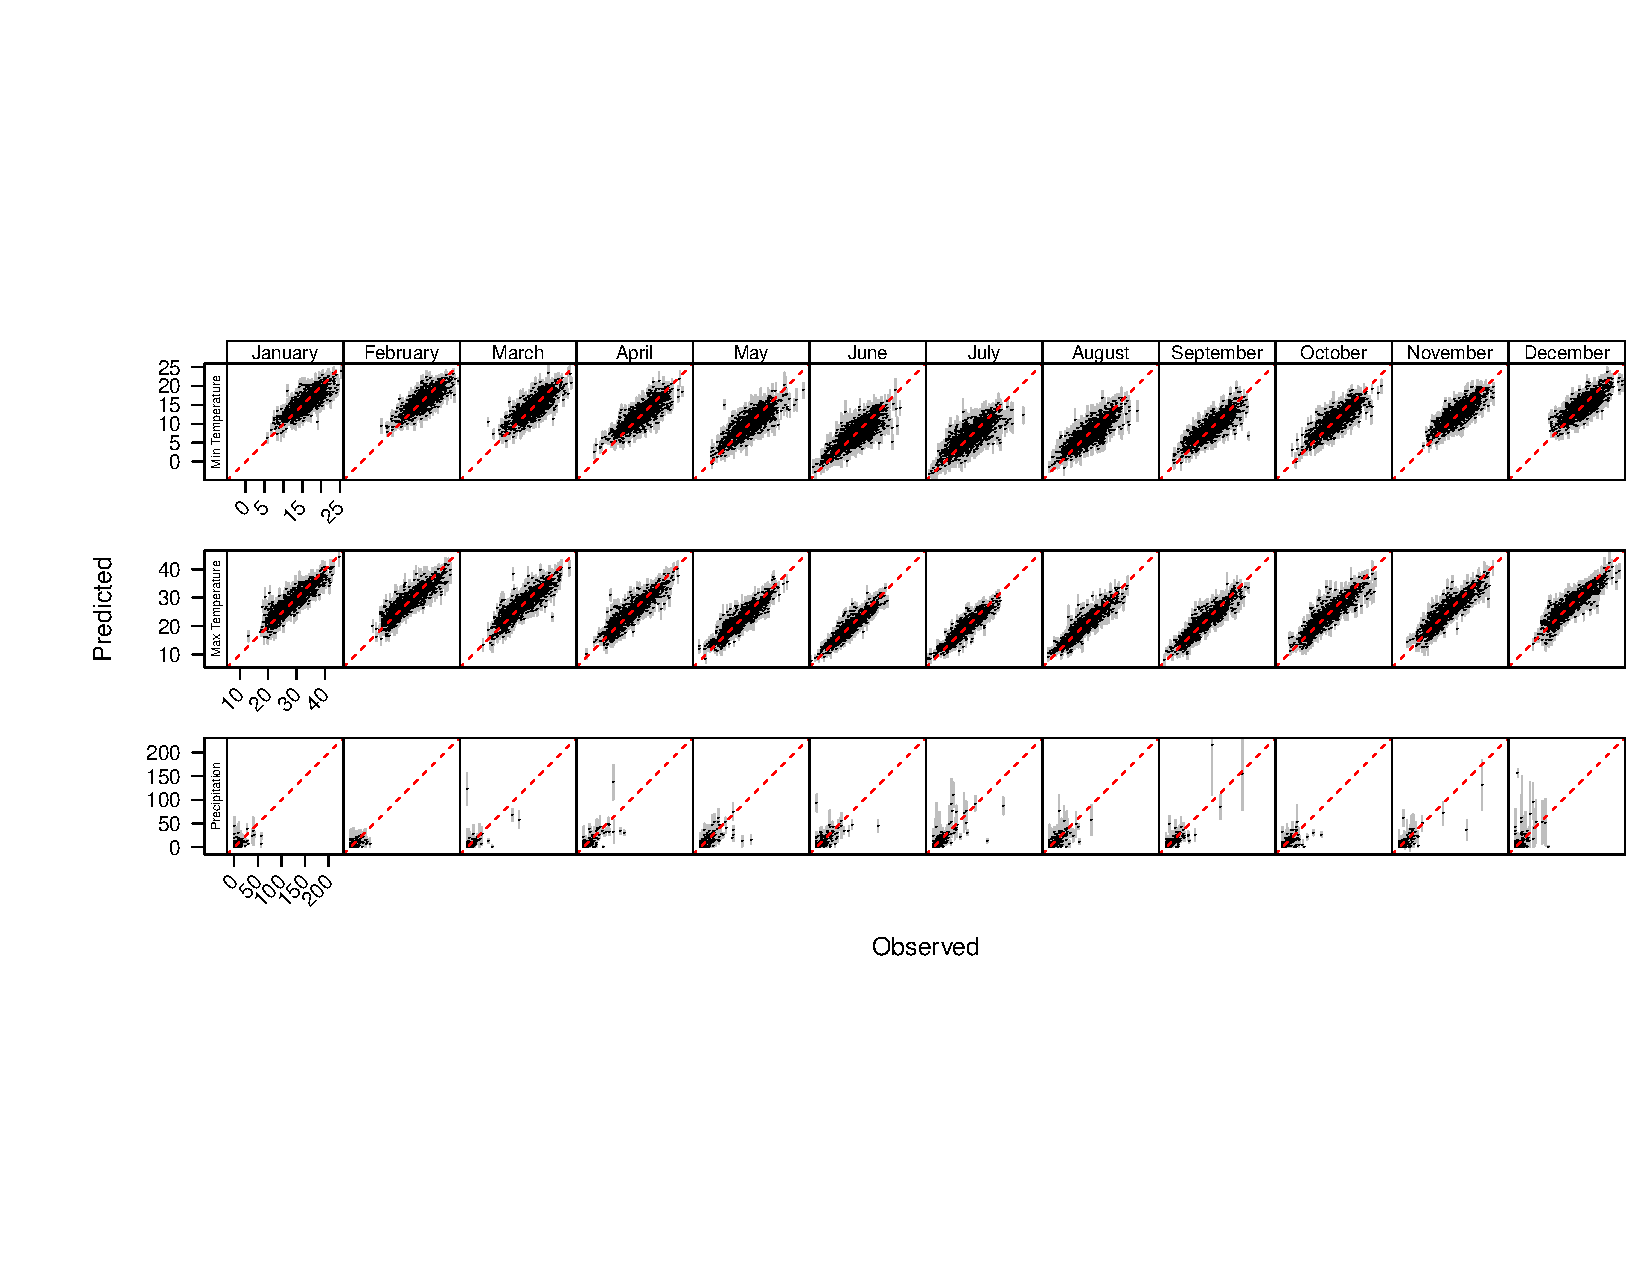
\includegraphics[clip=true,trim= 1mm 4.8mm 0 5.2mm,width=\textwidth]{Figure4.pdf} \caption{Scatterplot of
   predicted and observed weather from the daily hold-out validation
   stations separated by month (columns). The units for both $x$ and $y$ axis
   are $^o$C for temperature and mm for precipitation.  Grey bars represent $\pm1$ standard deviation of the posterior
   distributions. The dashed lines indicate $y=x$.}
    \label{fig:predobsm}
\end{center}
\end{figure}
%\end{landscape}

\subsection{Validation of Monthly Data}

The validation of the monthly data resulted in lower predictive accuracy than
the validation of the daily data for maximum and minimum temperature (R$^2=0.60$
and R$^2=0.48$, respectively), but a similar value for
precipitation (R$^2=0.56$, Table \ref{tab:valid}).  
The lower correlations for temperature are expected because the weather stations recorded the
absolute minimum and maximum temperature (rather than the monthly mean of the
daily extremes) and are thus sensitive to a single day's value.  
The precipitation data, on the other hand, represent the monthly sum and so
the comparison is less sensitive to each day's value. 

\subsection{Spatial and temporal variability of uncertainty}

This interpolation method results in full posterior distributions for
daily minimum temperature, daily maximum temperature, and
precipitation.  
These distributions can be used to derive any quantities of interest from the daily weather values to any derived climate
metric. 
For example, Figure \ref{fig:CDD} shows the posterior mean and
coefficient of variation (CV, $\frac{\sigma}{\mu}$) of the longest period of consecutive dry days (CDD) across
the region for the year 2000.  CDD is a critical climate metric
affecting plant survival and reproduction and hence distribution in
some ecosystems \citep{kimball_fitness_2012}. 
In this plot, the contours reveal the complex topography of
uncertainty in the posterior distributions of cumulative dry days.
Note the complex `ridges' of uncertainty that exist between stations.  
The inset plot shows the relationship between the mean and CV.  
The arc-like structures are a function of distance to the nearest
station.  
The mean and CV of four
climate metrics representing extremes in both temperature and
precipitation for the year 2000 are shown in Figure \ref{fig:metrics}.  
The longest period of consecutive dry days (CDD) tends to be higher in the north-eastern mountains and arid interior and
lower in southern coastal regions while the CV tends to have depressions in locations near stations.  
The longest period of consecutive frost days (CFD) is higher in
interior mountains and lower in coastal areas in contrast to the CV of
CFD, which tends to be low in the mountains and higher in the coastal
areas. 
The lower elevations in the northwest portion of the region has more consecutive summer days (CSU) than the
southeast.  
The number of large precipitation events (ECA) is highest in the
southeastern mountains and eastern coastal areas, and lowest in the
arid interior. 
The posterior distributions of the predictions for climate metrics in each year at both of the example locations shown in Figure
\ref{fig:wmap} are illustrated in Figure \ref{fig:nearfar}.  
The within-year variability represents uncertainty about what the
`true' value was for that location in that year.  
In Figure \ref{fig:nearfar} it is clear that there are significant
year-to-year differences across the various metrics.  Some years
(\textit{e.g.} 1999)  are warm and dry at both sites while some years
(\textit{e.g.} 1996) are cooler and wetter.
As several of the metrics are sensitive to the events on a single day
(such as CDD and CFD), there can be considerably more uncertainty in
the estimated value and that uncertainty can vary from year to year.
For example, the mean estimated CDD for the Cederberg location in 1994
(69 days) was similar to 1997 (66 days), but the
inter-quartile widths (IQW; 2.5\%--95\%) were 10 and 33 days, respectively
(Figure \ref{fig:nearfar}). In contrast, the mean estimates for the Table Mountain
location in 1994 and 1997 were both 17 days, while the IQW's were 16
and 10 days, respectively.  
The differences in the variance of the predictions for the two
locations are primarily due to Table Mountain's location in an area with
ten stations within 3km, while the Cederberg site's closest station is
more than 10km away.  
These metrics are much more sensitive  than long-term or even monthly means to infrequent extreme climate
events that are critical to explaining the occurrence and distribution of species across a region. 

 %  \centering
     \begin{figure}
  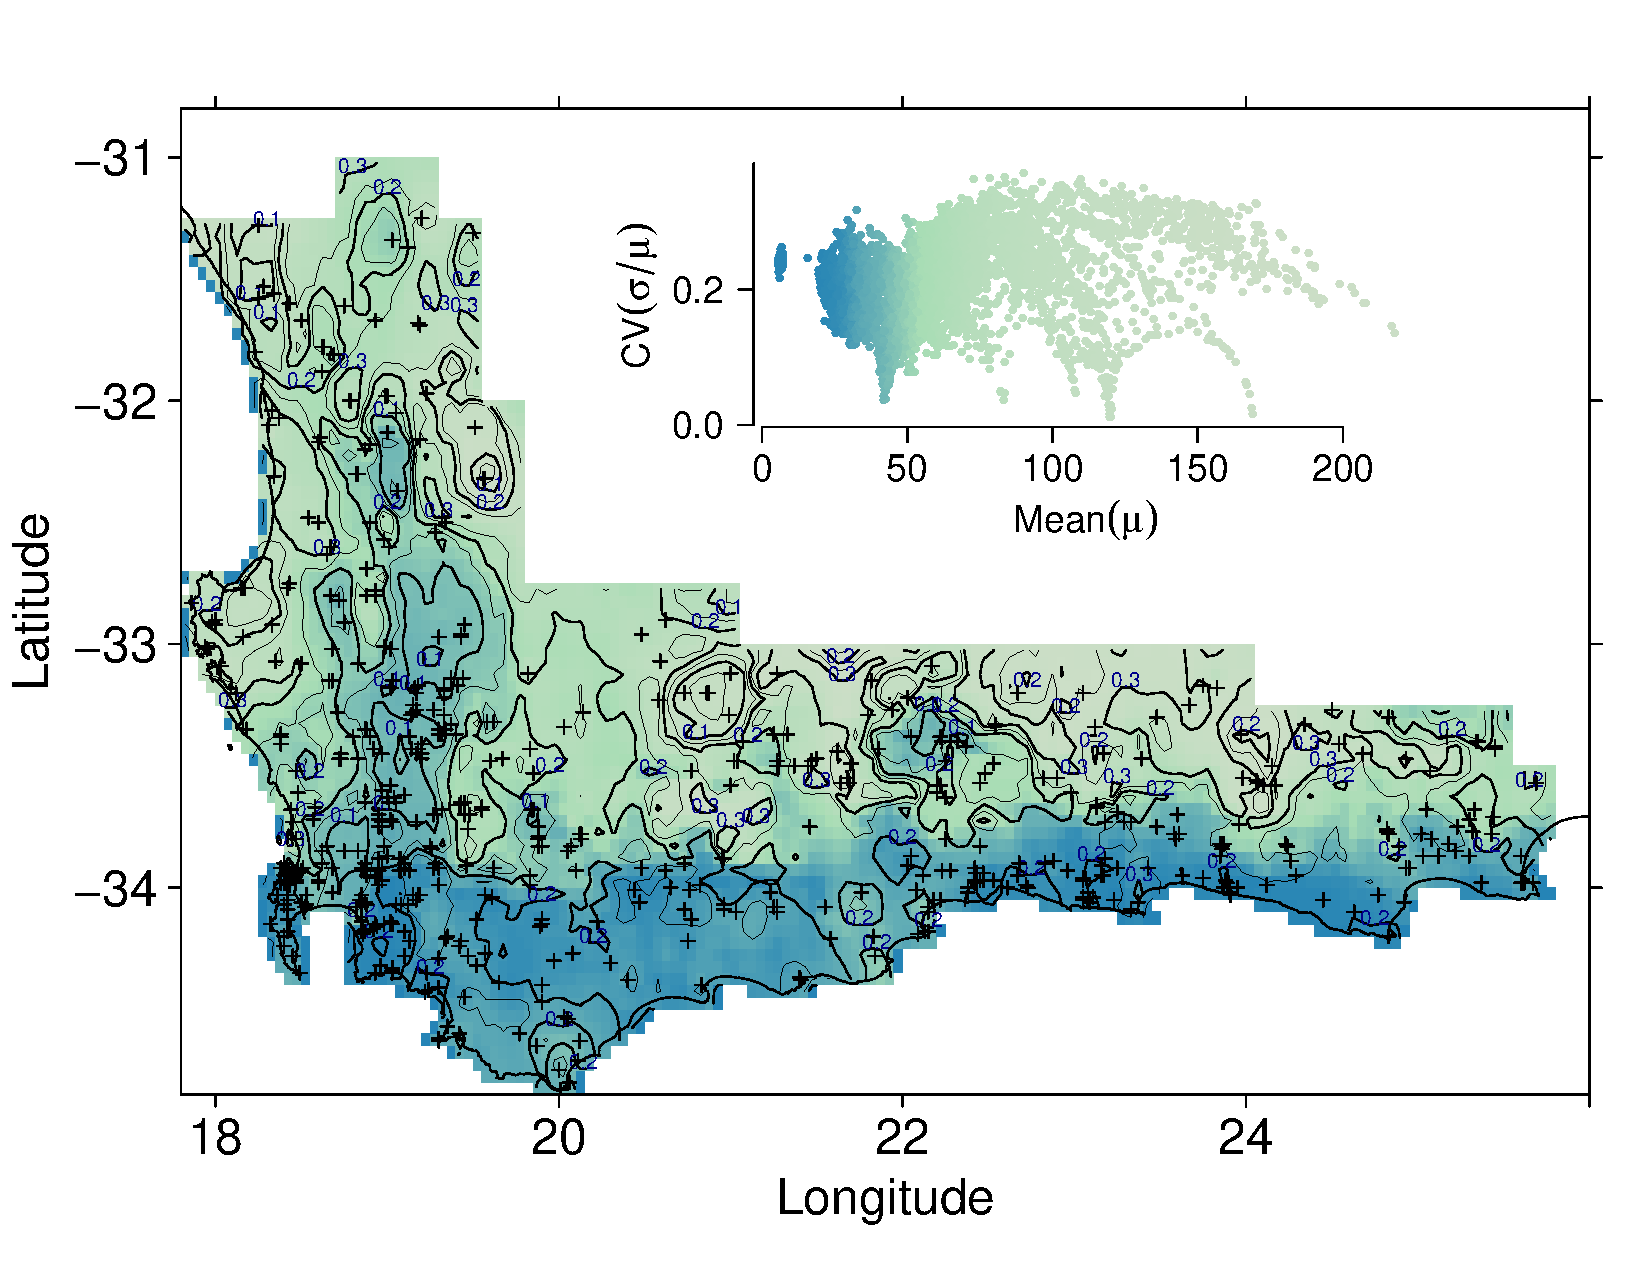
\includegraphics[width=\textwidth]{Figure5.pdf} \caption{Map
    illustrating the longest period of cumulative dry (precipitation
    $<2$mm) days for the year 2000. Mean posterior values are shown in
    shades of grey with the coefficient of variation (CV) of the posterior
    distributions ($\frac{\sigma}{\mu}$) overlaid as contours.
    The inset plot shows the relationship between the mean
    posterior values and the CV and serves as a key for the map. 
    The arcs are a function of distance to the
    nearest meteorological station, with lower coefficient of variation in pixels close to
    stations.  
    The white crosses indicate locations of
    meteorological stations with data used in the interpolation. Note
    that between stations in drier areas there are often `ridges' of
    uncertainty, while in wetter areas the uncertainty is lower due to
    frequent precipitation events. }
     \label{fig:CDD}
\end{figure}

%\begin{landscape}
% \centering
     \begin{figure}
  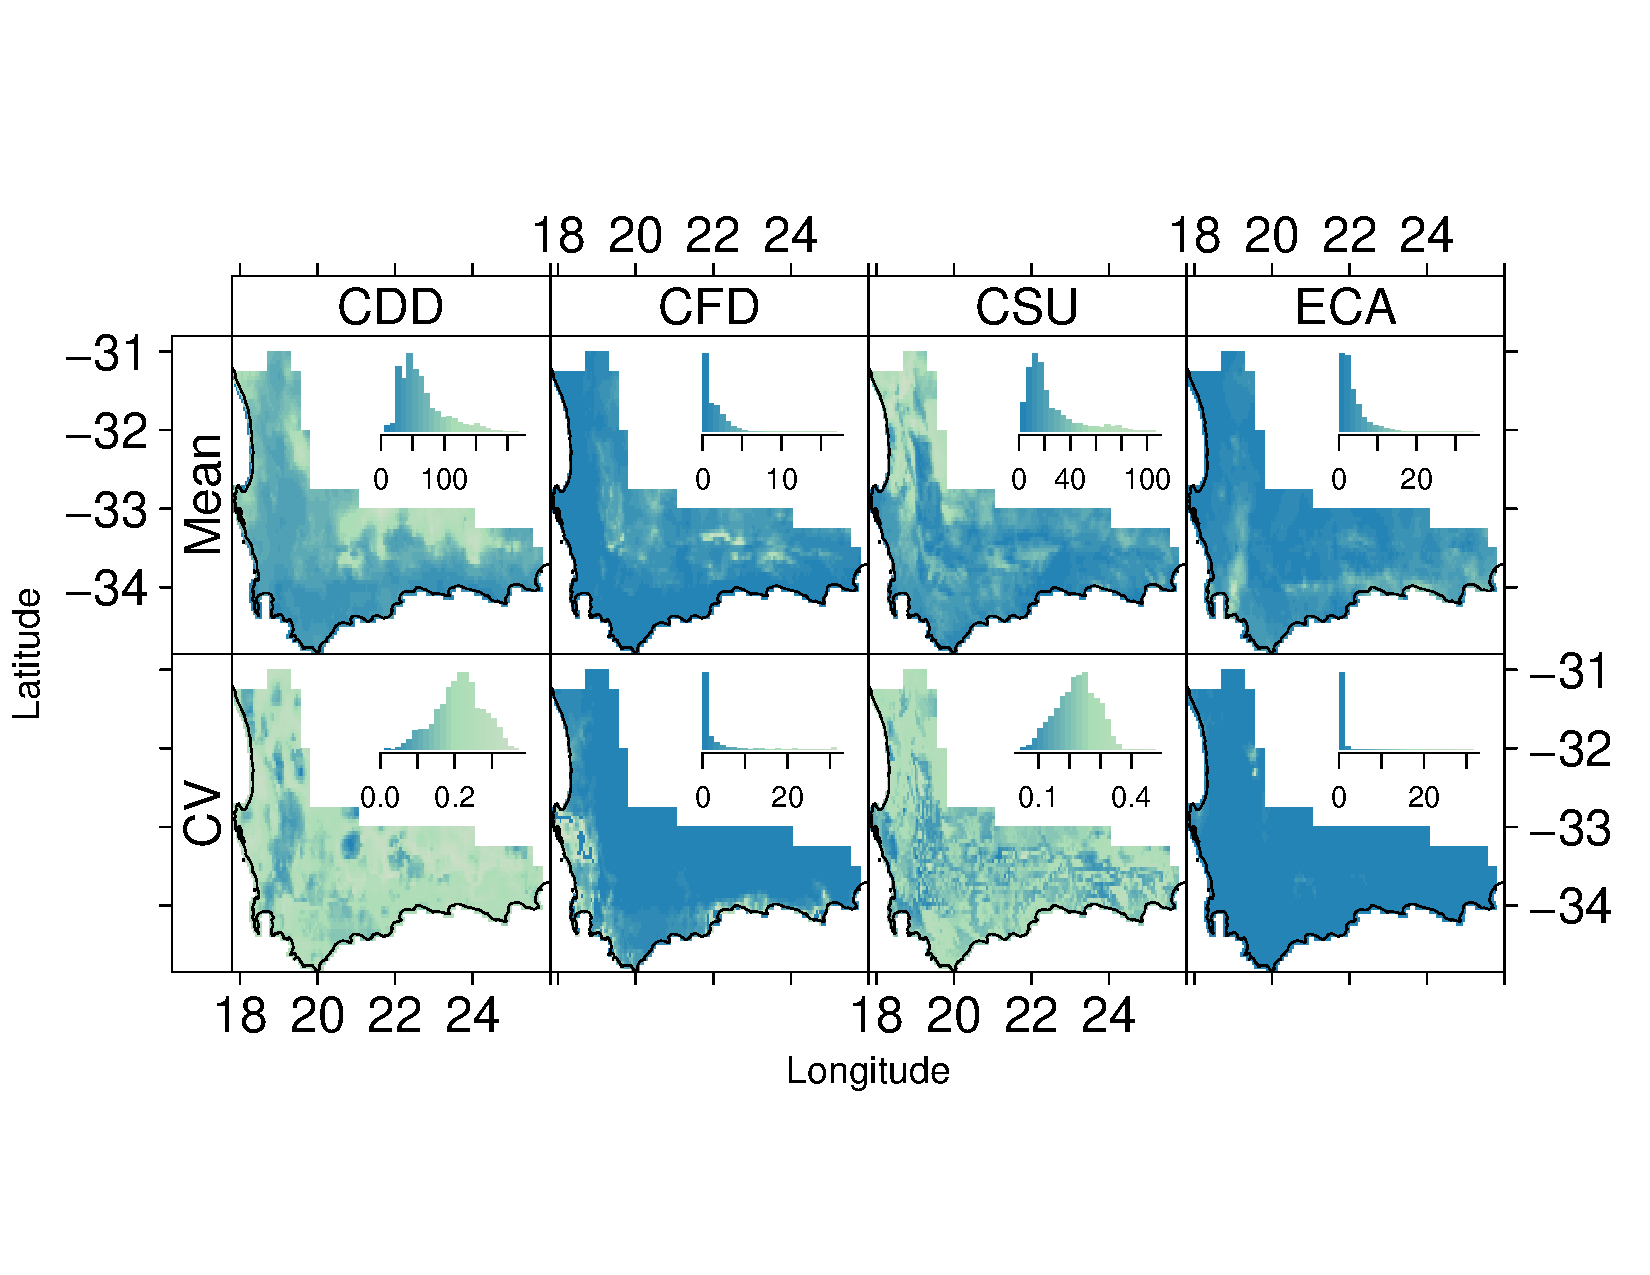
\includegraphics[width=1\textwidth]{Figure6.pdf} \caption{Maps
    illustrating the mean (top row) and coefficient of variation (bottom
    row) of the posterior  samples for four climate metrics for the
    year 2000:
    consecutive dry days (CDD), consecutive frost days (CFD),
    consecutive summer days (CSU) and the number of rain events
    $>20$mm (ECA).  
    See Table \ref{tab:climmet} for a description of each metric. 
    The histograms show the distribution of values within each panel. 
    Note that the coefficient of variation of the predictions is a complicated function of
    distance to the nearest station and the predicted value.  }
     \label{fig:metrics}
 \end{figure}
%\end{landscape}


\begin{figure}
  \begin{center}
    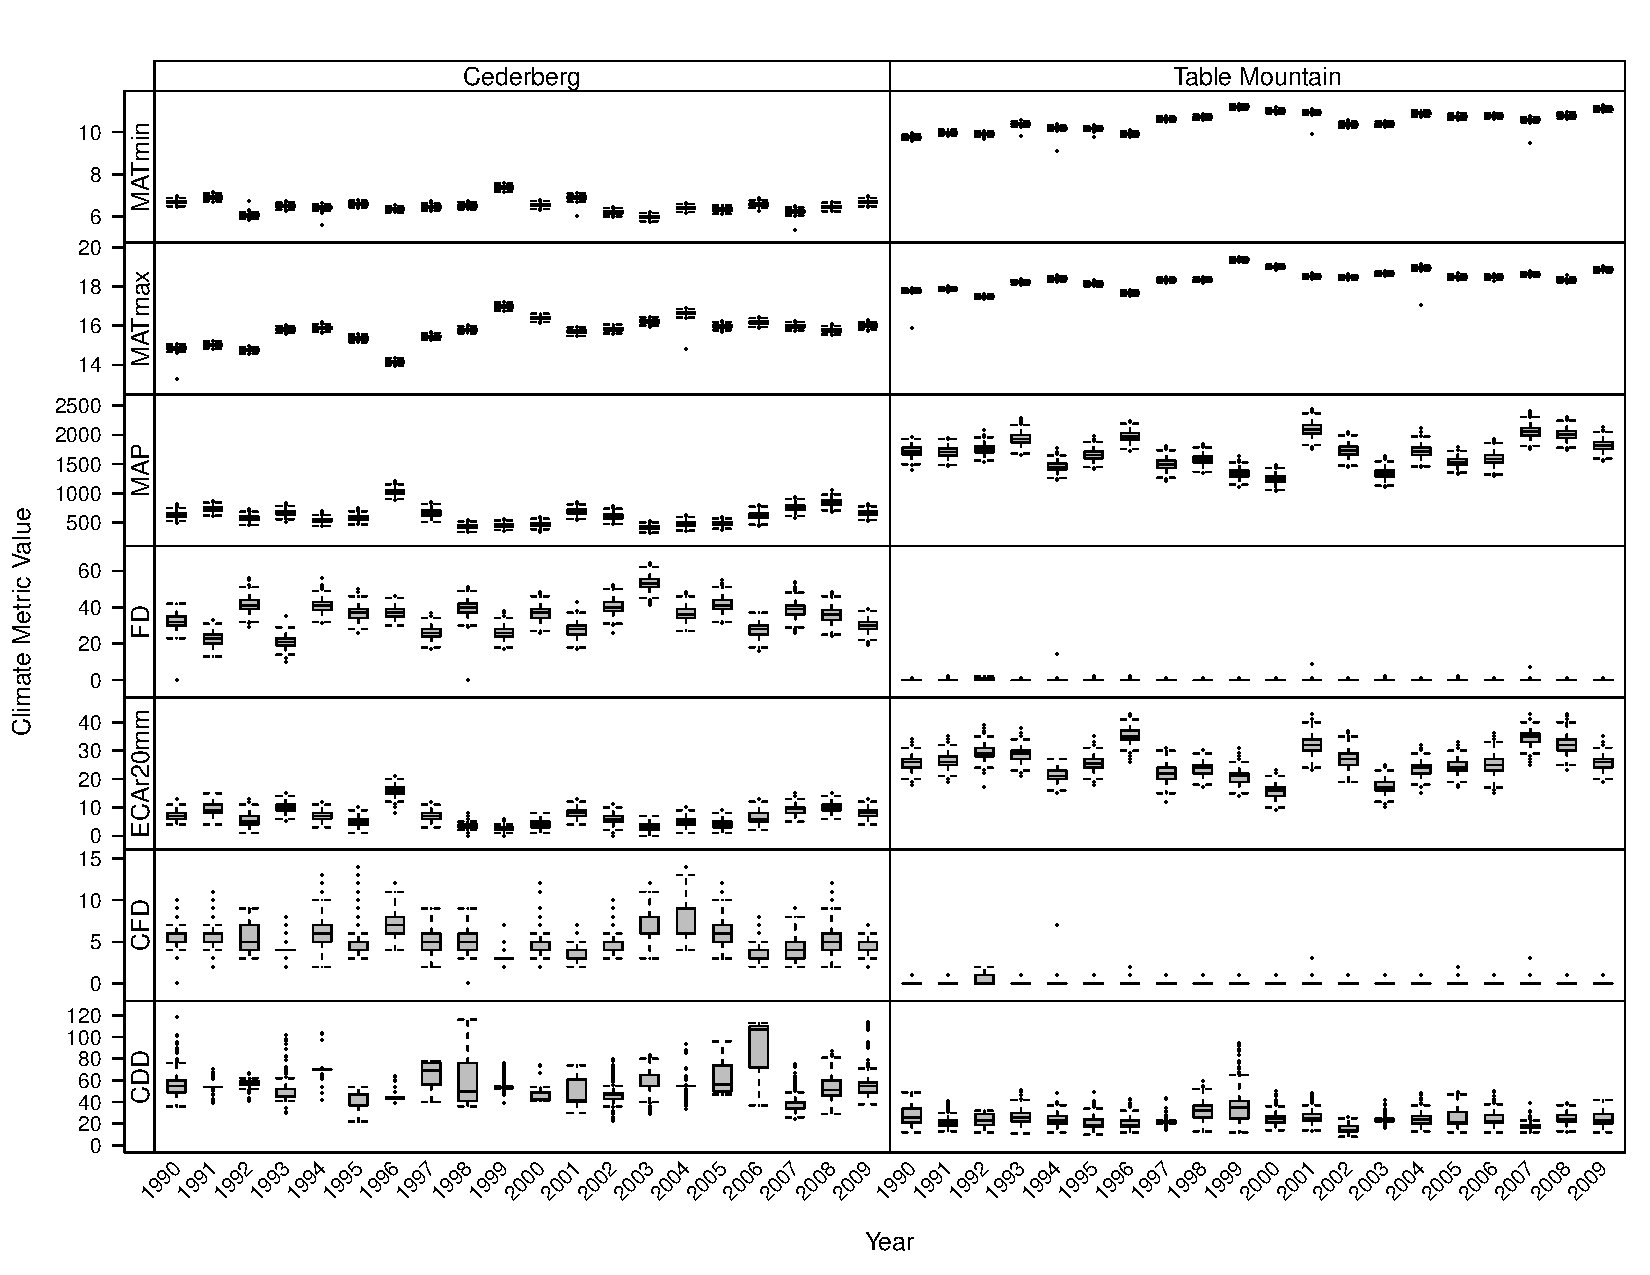
\includegraphics[page=1,width=\textwidth]{Figure7.pdf} \caption{Comparison
 of the posterior distribution of the climate metrics (see Table \ref{tab:climmet})  for two locations
 (Cederberg and Table Mountain, see Figure \ref{fig:wmap}).  Variables include: mean annual minimum temperature (MATmin, $^o$C), mean annual maximum temperature (MATmax, $^o$C), mean annual precipitation (MAP, mm),  number of frost days (FD), the number of rain events $>$ 20mm (ECAr20mm), consecutive frost days (CFD), and consecutive dry days (CDD).  Table
 Mountain has ten stations within 3km, while the Cederberg's closest
 station is over 10km away.}
    \label{fig:nearfar}
\end{center}
\end{figure}

\section{Discussion}

The uncertainties in the climate metrics reflect sparseness in weather
station data along with complexity in landscape topography and the
metrics themselves.
If meteorological observations were available for every square kilometer across the
region, there would be little spatial variability in the uncertainty in any interpolation at a
comparable resolution.
Likewise, if the topography were flat and the weather driven primarily by
large frontal systems, an equivalently sparse weather
station network would yield lower uncertainty than in topographically-heterogeneous landscapes. 
The results illustrate the value of quantifying the uncertainty of
interpolated weather surfaces across space and time. 
It is possible that changes to the modeling structure (such as
altering the spatial decay function) or priors could improve the predictive
performance of this model for this set of data, but predictive
uncertainties will always be present in any interpolated surface.  
Our intention here was to demonstrate an interpolation method capable
of propagating interpolation uncertainties through to
the final estimates of ecologically relevant climate metrics.  

The maps in Figure \ref{fig:metrics} illustrate that even in a region
of the world with a relatively high density of reliable weather
stations, there is still considerable uncertainty in the interpolated
predictions (whether or not the uncertainties are estimated).
Furthermore, the spatial uncertainty in the interpolated climate metrics is a
complicated function of distance to the nearest station and the
properties of the metric itself.  For example, note the extreme spatial variability of the CV of CDD in Figure
\ref{fig:CDD}.  South of 34$^o$S, the CV surface is relatively
smooth while north of 34$^o$S, the surface is very irregular and
highly sensitive to the locations of stations.  Because the inland
areas are more arid, there is greater potential for a large CDD and
thus locations far from stations have large uncertainty in the
predicted values.  
In contrast, southern coastal areas (which receive more regular rainfall)
have both lower CDD and associated CV, even in areas far from
stations (\textit{e.g.} 21$^o$E, 34.5$^o$S).


\subsection{Implications of climate data uncertainty in
  ecological modeling}
Ecologists are under increasing pressure to make predictions about
ecological change \citep{clark_ecological_2001}.
Detecting, attributing, and predicting ecological change requires techniques
that carefully account for the uncertainty inherent in an increasing variety
of data sources including traditional field observations, remote
sensing \citep{muraoka_satellite_2009}, embedded sensor networks
\citep{collins_new_2006,clark_inferential_2011}, and interpolated climate data
\citep{soria-auza_impact_2010,roubicek_does_2010}. 
The intention of this study was to illustrate how a
Bayesian framework can propagate the uncertainty in
interpolations of daily meteorological data through to the final
surfaces of ecologically and biologically relevant climate metrics and provide
posterior distributions that can later be incorporated into ecological analysis.  

Previous work has revealed that the choice of weather data can make a
significant impact on the results of ecological analysis.  For
example, Soria-Auza, et
al. (\citeyear{soria-auza_impact_2010}) used the MaxEnt framework
\citep{elith_statistical_2011} to compare estimate species
distributions using climate data available via WorldClim \citep{hijmans_very_2005} and SAGA
\citep{bohner_advancements_2005}.  
Even though the differences these datasets were relatively minor
(correlations ranged from 0.46 to 0.99 across climate variables), the
authors reported significant differences in the predictions in some regions.  
In a similar fashion, Peterson and Nakazawa
(\citeyear{peterson_environmental_2008}) compared species distribution
models for fire ants (\textit{Solenopsis invicta}) developed using climate data from three sources: WorldClim
\citep{hijmans_very_2005}, the Hadley Climate Model \citep{johns_second_1997}, and the Center for Climate Research at the
University of Delaware \citep{feddema_revised_2005}.  
They found significant differences in the predicted distributions
developed using the various climate data sets.  
In both of these studies, the authors used additional information to assess the
relative merit of the predictions derived from various climate data
(WorldClim performed worse in both cases).  
However, it is common in distribution modeling studies that no
independent climate data (or interpolation uncertainties) are available and thus
ecologists are faced with either arbitrarily choosing a climate
dataset or making predictions with multiple climate datasets and
noting the differences.  

The situation is similar to the use of output from global climate models
(GCMs).  
Typically the output from multiple GCMs are treated independently in ecological analysis \citep[e.g.][]{beaumont_why_2008,lawler_projected_2009} and the
differences are explored by comparing the resulting predictions.
Alternatively, sometimes the mean of several GCMs are used \citep{ahmed_bias_2013}. 
This is  analogous to the independent comparisons of different climate interpolations
mentioned above.  
There has been some recent effort to develop probabilistic climate
projections by treating output from different GCMs as `samples'
from a `true' future climate \citep{tebaldi_use_2007} which would
allow probabilistic ecological projections.  
This approach has not yet been widely adopted, in part because the
uncertainties in the output  from GCM ensembles are
difficult to quantify due to lack of verification and model
dependence, bias, and tuning  \citep{tebaldi_use_2007}. 
In contrast, the uncertainties inherent in interpolating climate data from station
observations are much more tractable and the methodology presented
here results in probabilistic spatio-temporal estimates that can be
incorporated into further ecological analysis.  

For example, recent developments in Bayesian species distribution
models are capable of incorporating co-variate data into the model as a random variable and thus account for the
uncertainty of the data in the results. See \citet{chakraborty_modeling_2010,chakraborty_point_2011} and \citet{mcinerny_fine-scale_2011} for
examples of species distribution models that could incorporate the
uncertainty of the climate metrics via Markov chain Monte Carlo
sampling.  
Propagating this uncertainty could be achieved relatively easily by
considering the environmental variables to be random variables and
sampling from their interpolated posterior distributions in each
iteration of model fitting.
For example, consider a simple linear regression that could be used
to explain ecological performance (such as the growth or reproduction
of individuals across space or time) as a function of its environment,
$\boldsymbol{y}\sim\mathcal{N}(\boldsymbol{X\beta},\sigma^2)$ where $\boldsymbol{y}$ is a vector
of $i\in1:I$ observations of performance in different locations/times and $\boldsymbol{X}$ is a $I\times P$
matrix of P co-variates for each location/time.  Typically the matrix of
explanatory variables ($\boldsymbol{X}$) is considered to be known
exactly even when, as is usually the case, the data have associated uncertainties.  
By adding another level to the model which samples the $\boldsymbol{X}$'s from a distribution (such as the
climate metrics described in this paper),
$X_{I\times P}\sim\mathcal{N}(\mu_{I\times P},\sigma_{I\times P}^2\mathcal{I}_{I\times P})$, the uncertainty in the environmental variables will
be propagated through to the predictions of the model.         A similar approach has been recently explored in epidemiological models
that combine algorithmic models with stochastic exposure simulators to estimate
human exposure to toxins \citep{gelfand_combining_2010}.    Surprisingly, propagating uncertainty in this way is exceedingly rare in ecology.     A notable exception is the work of \citet{mcinerny_fine-scale_2011}, which provides an interesting application of a hierarchical species distribution model to account for both environmental uncertainty (measurement error) and sub-pixel variability.  They found that adding a latent variable for the `true' (but unknown) environment actually reduced regression dilution by allowing sub-pixel environmental variability and enabled improved predictions of species distributions.  Furthermore,  multi-species models with common latent environmental variables  dramatically improved model performance by increasing the constraints on both latent variables and species parameters.  Climate data that include careful quantification of uncertainties, such as those produced in this study, should  facilitate the development of a richer and more robust predictive modeling in ecology and biogeography.  

\subsection{Potential Enhancements}
The methodology presented here could be further enhanced in several
ways. For example, due to computational limitations we were limited to
interpolating the anomalies at $^1/_4$ degree resolution even over
this relatively small region.  Use of a ``predictive process'' spatial
model \citep{banerjee_gaussian_2008}
to decrease the size of the spatial covariance matrix would facilitate
increasing the size of the region (and number of stations) while still
accounting for spatial autocorrelation \citep{chakraborty_point_2011}.  
Additionally, our method ignores the uncertainty present in the underlying
interpolated long-term climate surfaces.  This was unavoidable because
no uncertainty estimates were available \citep{schulze_south_2007} which is usually the case for long-term climate summaries.
Future analyses could rectify this situation by first generating high
resolution climate surfaces (with uncertainty estimates) prior to
interpolating daily anomalies.  It would also be possible to
incorporate other sources of information at either the
climatic or daily anomaly stage, including topographic variables, distance to nearest coast, land cover type, satellite observations of temperature or clouds \citep[\textit{e.g.}][]{alvarez-villa_improved_2011,hart_daily_2009} or results from a
coarse-grained reanalysis of global meteorological data
\citep[\textit{e.g}][]{compo_twentieth_2011}.  

\section{Conclusion}
Various methods have been employed to understand how environmental
change will impact biodiversity, including models of species
distributions \citep[e.g.][]{franklin_modeling_2012} and demographic processes
\citep[e.g.][]{jenouvrier_effects_2012}.  Typically, practitioners 1) fit a
model using historical explanatory data, which often includes
interpolated climate data and/or remotely sensed products and then 2)
use that model to project into the future using climate model
output. In other words, models constructed to forecast biodiversity
often use `output' from other models as `input' data.  However, in
most cases the uncertainties presented in the results are derived only
from the biological model and ignore uncertainties in the source
datasets.  Statistically, this is a reasonable approach with the
important caveat that the results are conditional on the input
datasets.  But for decision-making purposes, it is important that the
uncertainties represent the overall confidence in the forecast.  The
IPCC, for example, has standardized how uncertainties should be
handled and described throughout their publications
\citep{mastrandrea_guidance_2010} and other disciplines, such as
hydrology, have taken this problem seriously \citep[e.g.][]{Liu_uncertainty_2007}.   Thus ecologists are
faced with the important challenge of propagating uncertainties
inherent in source datasets through new models to the final results.
In this study we introduced a method to generate continuous surfaces of
ecologically relevant climate metrics that include estimates of
uncertainty introduced by the interpolating from station values.  We
also presented  a simple example of how this sort of data could be
used in a hierarchical distribution model to further propagate the
uncertainty through to ecological predictions.  
The methodology presented here could have wide application for
ecological models capable of incorporating and propagating data
uncertainty through to the model output and results.  This will likely lead to projections with
wider prediction intervals that we can be more confident in.  

\singlespacing
\bibliographystyle{humanbio}
\bibliography{/Users/adamw/biblio}
\doublespacing

\end{document}
